\documentclass[thesis.tex]{subfiles}

\begin{document}

% ----------------------------------------------------------
\chapter{Introduction} \label{chap:introduction}
% ----------------------------------------------------------
Explain the aims and rationale for the physics case and what you have done. At the end of the introduction you should give a brief summary of the structure of the report. Motivate the reader and give overarching ideas. Describe what has been done and the structure of the report (how is it organized).
% ----------------------------------------------------------

% ----------------------------------------------------------
\section{Background and Motivation} \label{sec:background_and_motivation}
% ----------------------------------------------------------
\textbf{** This entire section is going to be rewritten **} \bigbreak \noindent
In this project we aim to design and develop a system for analyzing medical videos from a camera pill, as seen in Figure \ref{fig:pill-cam}. The pill is swallowed and records video of the entire digestive system The goal is to be able to detect different irregularities in the patients digestive system, like a colon polyp, Chron's disease, Colorectal cancer, etc. by using video object tracking, object detection, machine learning or other relevant tools.

Neural networks models that we would like to explore further for this purpose are Convolutional neural networks (CNN), Recurrent neural networks (RNN), Capsule neural networks, Long Short-Term memory networks and more.

The main idea is to go beyond image-based methods and also exploit the time factor of the data. 
The videos we will be using for this is delivered by Bærum Hospital, and is carefully labeled by using tools such as described in the paper \citetitle*{ExpertDriven15}. In this paper \citeauthor*{ExpertDriven15} presents a semi-supervised method to gather the annotations in a easy and time saving way \cite{ExpertDriven15}.

%TODO : remove image?
%TODO : source in footnote
\begin{figure}[H] % fig:pill-cam
  \begin{center}
    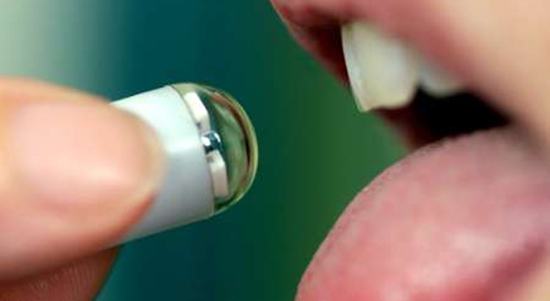
\includegraphics[width=0.9\linewidth]{pill-cam.jpg}
    \caption[Illustration of how such a camera pill could look like]{Illustration of how such a camera pill could look like\footnotemark.}
    \label{fig:pill-cam}
  \end{center}
\end{figure}

\footnotetext{\text{Image Credit: Medtronic}}


\subsection{Nomenclature used in the field of capsule endoscopy}
%Source: https://www.ncbi.nlm.nih.gov/pmc/articles/PMC4665909/
%TODO : move to WCE section? 
%TODO : correct all naming schemes in thesis this far
From a variety of literature searches we have found that there is five different terms in use:

\begin{itemize}
\item \textbf{VCE}: Video Capsule Endoscopy - capsule endoscopy including an imaging device such as a CCD (the capsule does not have to be wireless);
\item \textbf{WVE}: Wireless Video Endoscopy (not necessarily a capsule);
\item \textbf{CE}: Capsule Endoscopy - endoscopic capsule (not necessarily wireless);
\item \textbf{WCE}: Wireless Capsule Endoscopy (not necessarily containing an image sensor);
\item \textbf{WVC}: Wireless Video Capsule.
\end{itemize}

% created with: https://www.visme.co/
\begin{figure}[H] % fig:wce_nomenclature
  \begin{center}
    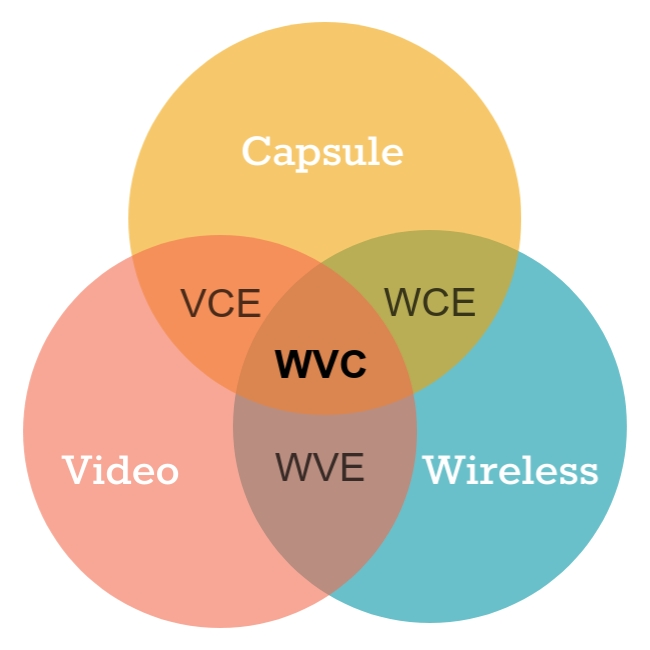
\includegraphics[width=0.5\linewidth]{wce_nomenclature.jpg}
    \caption[Distinction of the nomenclature relating to capsules, wirelessness and video.]{Distinction of the nomenclature relating to capsules, wirelessness and video.}
    \label{fig:wce_nomenclature}
  \end{center}
\end{figure}

The terms are often confused and used interchangeably. Consequently in this thesis they will all be referred to as WCE.



% ----------------------------------------------------------
\section{Problem statement} \label{sec:problem_statment}
% ----------------------------------------------------------
%TODO : add soure
Colorectal cancer (CRC) is the third most common cause of cancer mortality for both men and women \cite{CancerStatistics10}, and it is a condition where early detection is of clear value for the ultimate survival of the patient. As statistics show that 15\% of male and female above 50 years are at risk, the procedure is recommended on a regular basis (every 3-5 years) for the population over 50, and from an earlier age for high-risk groups. 

Colonoscopy is a demanding procedure requiring an significant amount of time by specialized physicians, in addition to the discomfort and risks inherent in the procedure. Traditional methods based on colonoscopy are not cost-effective for population-based screening purposes, so only about 2-3\% of the target population is reached at present. 

%TODO : add source for cost
The cost of a population screening program is prohibitively expensive. Colonoscopy is the most expensive cancer screening process in the US, with annual costs of \$10 billion dollars (\$1100 per person). In Norway we have similar costs of around \$1000 per person, with a time consumption of about 1 doctor-hour and 2 nurse-hours per examination. 

By researching an automatic system for a camera pill the aim is to greatly increase the number of patients that can be examined, i.e., making the public health care system more scalable and cost effective, while at the same time reducing the need for intrusive procedures like "bottom-up" examinations like colonoscopy.


% ----------------------------------------------------------
\section{Scope and limitations} \label{sec:scope_and_limitations}
% ----------------------------------------------------------
%Limitations tell you what you won’t do due to project constraints that form boundaries, while Scope tells you what will be done and gives a total overhead view of a doable project within a period of time..

% limitations: 
%- biased dataset coming from one source (hospital) and one sensor (pillcam). AKA low diversity in sample size
%- collecting data/segmenting findings done by untrained students with some guidance
%- time constraints
%- small sample size (few medical videos)
%- searching for a given set of diseases
%TODO : not knowing what the algorightm learns (unless implementing gradcam etc)
%TODO : temporal constraints due to low (and variable) frame rate

% scope: 
%- looking at only some AI models
%- compare atomatic classification systems against eachother
% ----------------------------------------------------------
Based on the described problem statement the scope of this thesis is to compare some prior selected automatic systems with focus on machine learning, for classification tasks in the medical domain. We will test the systems on video and still images taken from a wireless capsule endoscopy system, provided by Bærum Hospital. 
%TODO : fix VCE system
This data is collected with the Olympus Endocapsule 10 System\footnote{\url{https://www.olympus-europa.com/medical/en/Products-and-Solutions/Products/Product/ENDOCAPSULE-10-System.html}} and gives us a wide view of the GI-tract. A limitation for our research will therefore be that our dataset lack a great deal of diversity. While we might have a wide range of patients all the data contributions stem from one provider in one location. This might not be much of an issue due to GI-tract being quite homogeneous over large populations. But can presumably cause biasing issues in our deep learning models. % mention ethnicity and age

%TODO : needs to be rewritten to accomondate the changes made to the thesis
%TODO : write more aout augere medical
By using a tool provided by Augere Medical, we have sequentially classified each frame in XXX WCE videos, assisted by doctor Thomas de Lange, with many years of experience. To the best of our efforts we managed to divide the data into XXX classes which we later will train our networks on.

Considering the scope of this thesis, we will limit ourselves to use some of the more common deep convolutional neural networks and a more novel stacked hourglass network. There are many other more common network used in the field of object classification like NN, RNN, statistical methods, but these methods are widely tested and we wish to push the envelope of machine learning systems on medical videos and also have a wide variety of ways to score our model against previously tested algorithms.


% ----------------------------------------------------------
\section{Research methods} \label{sec:research_methods}
% ----------------------------------------------------------
%TODO : describe how our methodology fits into this

We have based this paper on Association for Computing Machinerys (ACMs) research
methodology. In the spring of 1986 ACM president Adele Goldberg and ACM Education Board Chairman Robert Aiken appointed a task force with the prime objective of describing the core fundamentals of computer science and computer engineering \cite{ComputingDiscipline89}. They introduced the phrase "discipline of computing" to embrace the two fields. The task force were given three objectives to complete.

\begin{enumerate}
\item Present a description of computer science that emphasizes fundamental questions and significant accomplishments. The definition should recognize that the field is constantly changing and that what is said is merely a snapshot of an ongoing process of growth.
\item Propose a teaching paradigm for computer science that conforms to traditional scientific standards, emphasizes the development of competence in the field, and harmoniously integrates theory, experimentation, and design.
\item Give a detailed example of an introductory course sequence in computer science based on the curriculum model and the disciplinary description.
\end{enumerate}

To fully elaborate the core fundamentals of computer science and computer engineering they agreed upon no core fundamentals is different in the two fields, but the difference is manifested in the way the two fields elaborate the core; computer science focuses mainly on analysis and abstraction and computer engineering focuses mainly on abstraction and design.

Furthermore the task force appointed three major paradigms which represent different areas of competence in the field. Some will argue that the different paradigms are implicitly based on an assumption that one of the three processes is the most fundamental, but as we will see, the three paradigms are so intricately intertwined that it is irrational to say that one is the most fundamental. The three paradigms, or cultural styles, are listed below.

\subsection{Theory} \label{sec:theory}
The first paradigm, Theory, is deeply rooted in mathematics and is concerned with the ability to describe and prove relationships among object. The paradigm consist of the following four steps.

\begin{enumerate}
\item Characterize objects of study (definition);
\item Hypothesize possible relations among them (theorem);
\item Determine whether the relationships are true (proof);
\item Interpret the results found.
\end{enumerate}

When working in this paradigm it is expected to follow this reasoning and iterate the steps when errors or inconsistencies are discovered, until they can be explained and interpreted.

\subsection{Abstraction} \label{sec:abstraction}
The second paradigm is abstraction. Abstraction is a form of modeling and is rooted in the experimental scientific method. This paradigm is concerned with the ability to use the relationships found in the theory paradigm to make predictions that then can be compared to the real world. It has four steps for which a scientist is expected to follow. 

\begin{itemize}
\item Form a hypothesis;
\item Construct a model and make a prediction;
\item Design an experiment and collect data;
\item Analyze the results.
\end{itemize}

\subsection{Design} \label{sec:design}
The third paradigm, design, is rooted in engineering and consist, like the others, of four main steps listed below. The design paradigm is concerned with the ability to implement specific instances of those relationships and use them to perform useful actions. The following four steps will help an engineer to construct a device or system to complete a given task.

\begin{itemize}
\item State requirements;
\item State specifications;
\item Design and implement the system;
\item Test the system.
\end{itemize}

An engineer is to iterate these steps until the results from the testing satisfy the requirements and specifications of the system.


% ----------------------------------------------------------
\section{Main Contributions} \label{sec:main_contributions}
% ----------------------------------------------------------
% what did your research contribute to the field?
% ----------------------------------------------------------
Write a section on how our work contributes to the field... TBW (to be written)


% ----------------------------------------------------------
\section{Thesis Outline} \label{sec:thesis_outline}
% ----------------------------------------------------------
% the layout of the thesis
% ----------------------------------------------------------
This thesis is split into five chapters. Chapter one and two are mostly to introduce the reader to the topic and to fill in the necessary knowledge to understand the rest of the thesis. In the last chapter we conclude on our findings and discuss our findings and propose further work. The papers that have been referenced in the thesis is added in the bibliography at the very end. The chapters in the thesis is summarized below:

%TODO : finish the chapter outline
\begin{itemize}
\item In Chapter \ref{chap:background} we discuss the literature that focus on the topic of automated lesion detection in computer systems.

\item In Chapter \ref{chap:methodology} we present the details of design, implementation of system and the processing and collection of data.

\item In Chapter \ref{chap:experiments} we present the experiments we have conducted and..

\item In Chapter \ref{chap:conclusions} we provide a comprehensive overview of the results found and discus what that contributes to the field and propose some further work.
\end{itemize}


\end{document}
